\documentclass{beamer}

\usepackage{graphicx}
\usepackage{amsmath, amsfonts, amssymb, amsthm} % For da math stuff
\usepackage{braket} % For sizeable brackets using \Set
\usepackage{mathpartir} % for the \inferrule command
\usepackage{booktabs}
\usepackage[normalem]{ulem}  % strike through text
\usepackage{color}

\newcommand*\esf[0]{\mathbf{E}_{S}^{f}} % Analogical extension
\newcommand*\esfs[0]{\mathbf{E}_{S}^{f*}} % Analogical extension star

\newcommand\eqdef{\mathrel{\overset{\makebox[0pt]{\mbox{\normalfont\tiny\sffamily
def}}}{=}}}
\newcommand*\rsfx[0]{\mathbf{R}_{S}^{f}(\mathbf{x})} % Analogical root of x
\newcommand*\albl[1]{\overline{f}(#1)}
\newcommand*\aroot[3]{\mathbf{R}_{#1}^{#2}(#3)} % Analogical root
\newcommand\given[1][]{\:#1\vert\:} %pour proba conditionnelle
\newcommand*\sol[0]{\text{sol}} % solution
\newcommand*\AD[0]{\text{AD}} % Analogical Dissimilarity
\newcommand{\norm}[2]{{\left\lVert#2\right\rVert}_{#1}} % Norm definition
\DeclareMathOperator*{\argmin}{arg\,min}
\newcommand*\nan[0]{1\text{-nan}} %pour 1nan
\newcommand*\nanemph[0]{1\emph{-nan}} %pour 1nan dans une def ou une prop
\newcommand*\knan[0]{k\text{-nan}} %pour knan
\newcommand*\knn[0]{k\text{-nn}} %pour knn
\newcommand*\NAN[0]{\mbox{NAN}} %pour NaN
\newcommand*\nn[0]{1\mbox{-nn}} %pour 1nn
\newcommand*\NN[0]{\text{NN}} %pour NN
\newcommand*\acc[0]{\mbox{Acc}} %pour Acc
\newcommand*\omegasf[0]{\omega_{S}^{f}} % omega
\newcommand{\aggr}[1]{\underset{#1}{\operatorname{aggr}}\;}
\newcommand{\predrui}{\hat{r}_{ui}}
\newcommand{\rui}{r_{ui}}


\usetheme{metropolis}

% Headline (TOC always on top)
\makeatletter
\setbeamertemplate{headline}{%
  \begin{beamercolorbox}[colsep=1.5pt]{upper separation line head}
  \end{beamercolorbox}
  \begin{beamercolorbox}{section in head/foot}
    \vskip2pt\insertnavigation{\paperwidth}\vskip2pt
  \end{beamercolorbox}%
  \begin{beamercolorbox}[colsep=1.5pt]{lower separation line head}
  \end{beamercolorbox}
}
\makeatother
\setbeamercolor{section in head/foot}{fg=normal text.bg, bg=structure.fg}

% Block style (else there is no background)
\metroset{block=fill}

\title{Contributions to the use of analogical proportions for machine learning}
\subtitle{Theoretical properties and application to recommendation}
\date{July 5, 2017}
\author{Nicolas Hug  ------ Henri Prade, Gilles Richard, Mathieu Serrurier}
\institute{Université Toulouse III Paul Sabatier - IRIT}
% \titlegraphic{\hfill\includegraphics[height=1.5cm]{logo.pdf}}

\begin{document}

\maketitle

\begin{frame}{Analogical proportion: \textit{a is to b as c is to d}}
  \begin{center}
  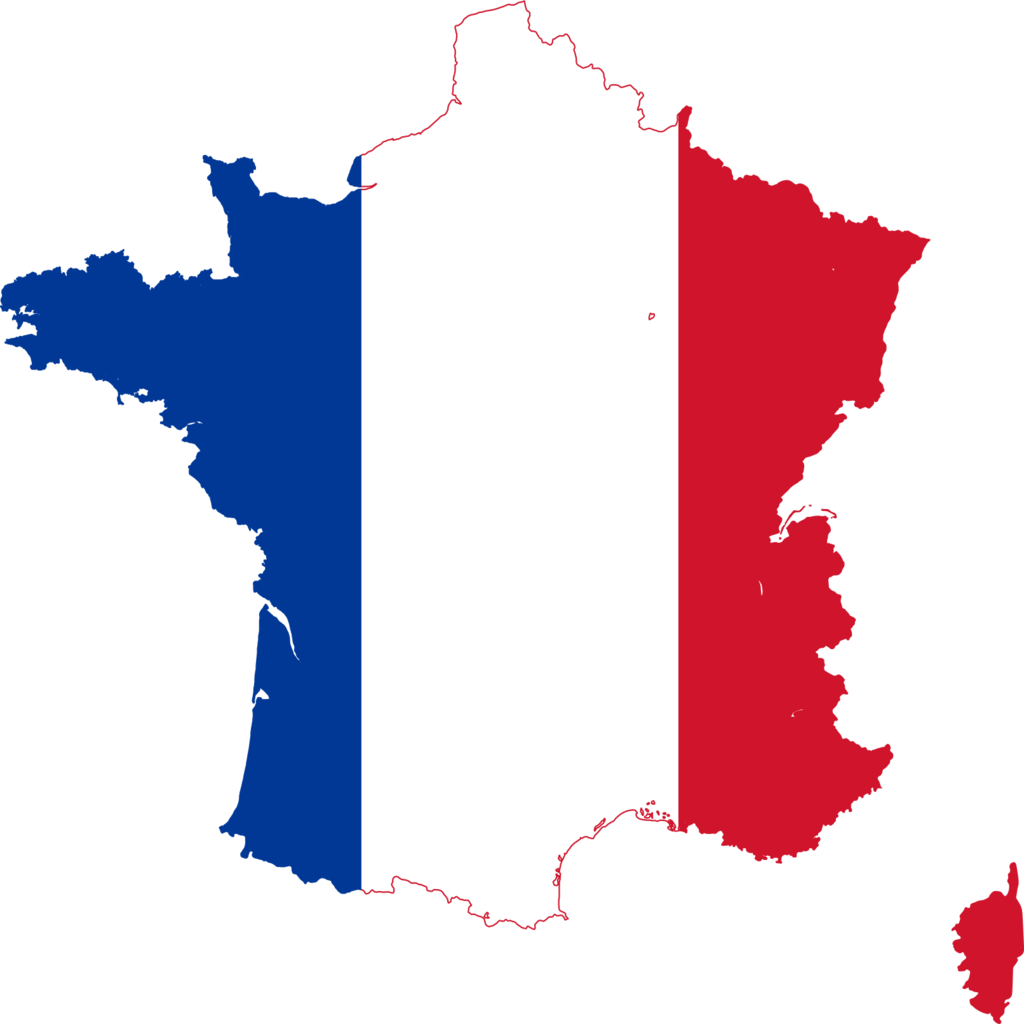
\includegraphics[width=0.17\textwidth]{figures/france.png}
  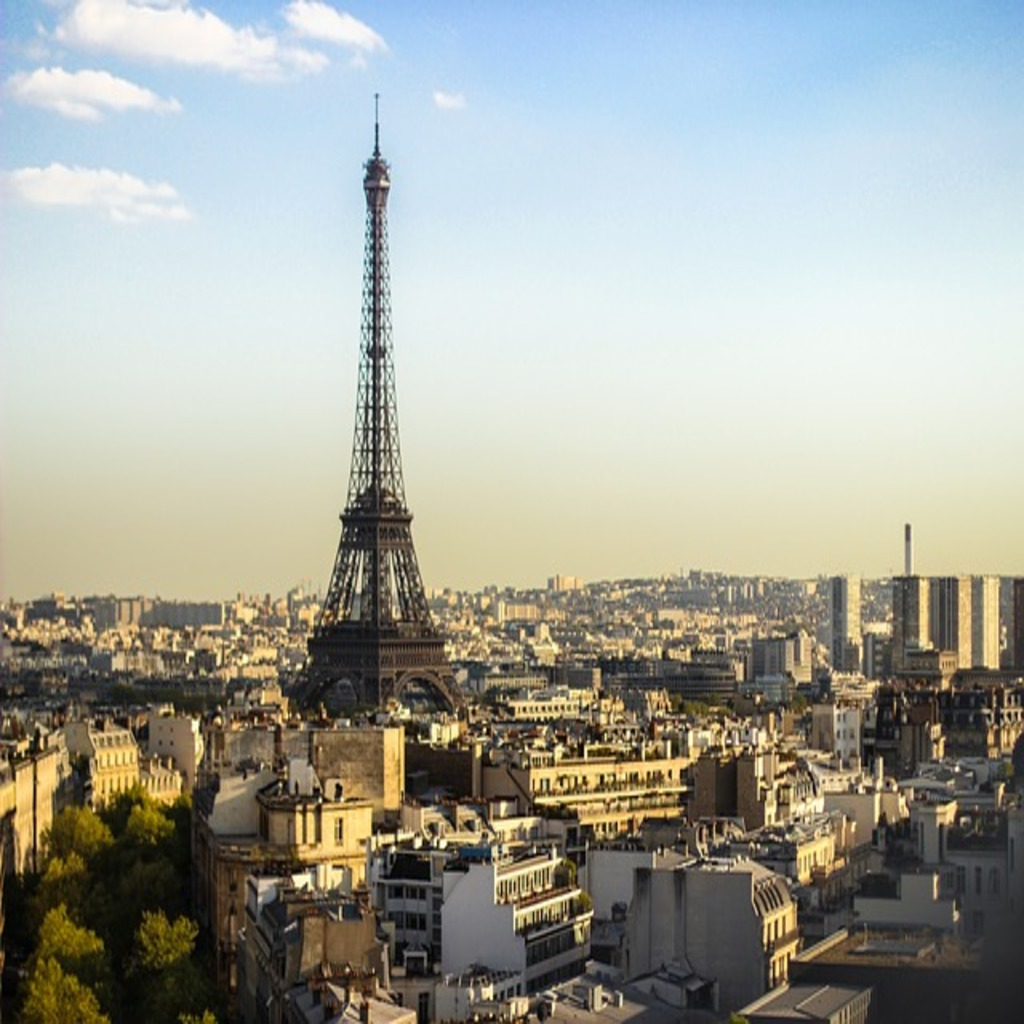
\includegraphics[width=0.17\textwidth]{figures/paris.jpg}
  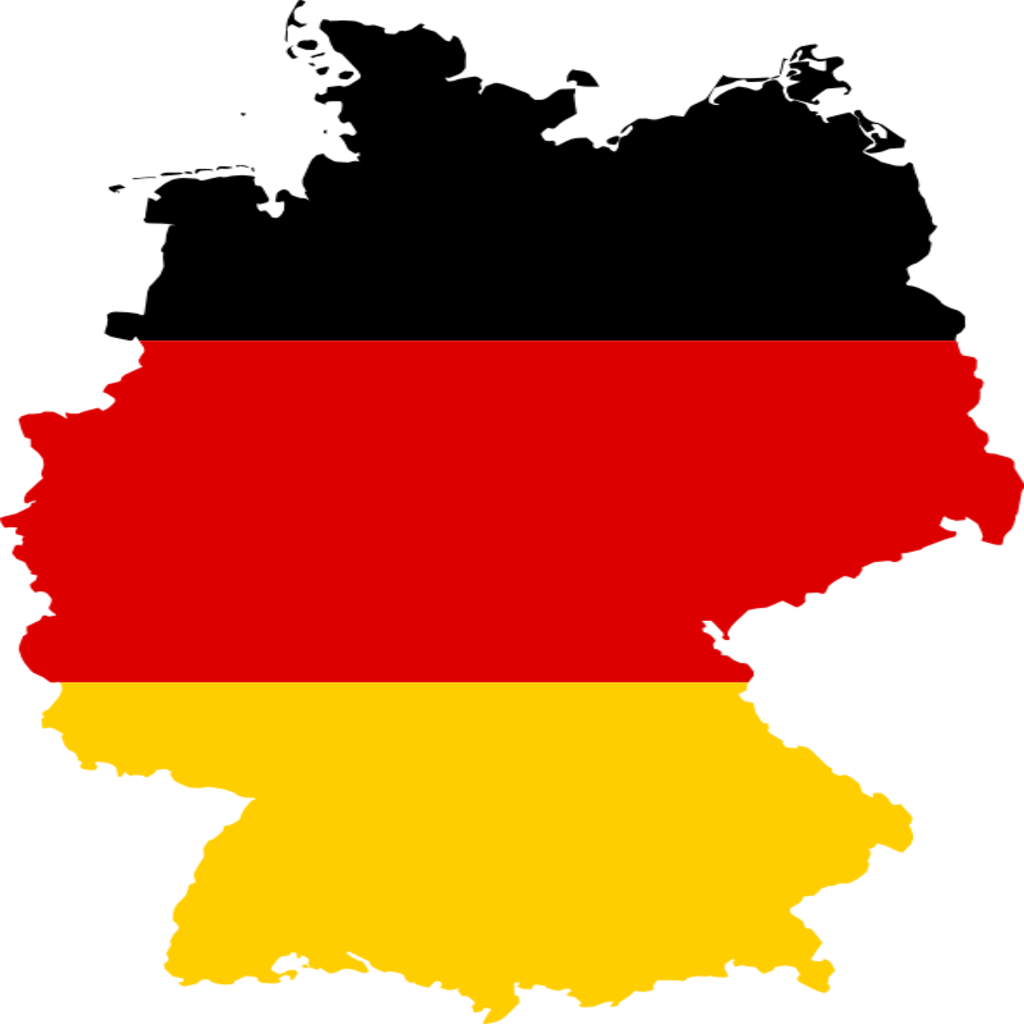
\includegraphics[width=0.17\textwidth]{figures/germany.png}
  
\includegraphics[width=0.17\textwidth]{figures/question-mark.jpg}
  \end{center}
  \begin{block}{Two key cognitive processes}
    \begin{itemize}
    \item Inference
    \item Creativity
    \end{itemize}
  \end{block}
  \begin{block}{Previous works in machine learning}
    \begin{itemize}
      \item Linguistics \cite{Lep03}
      \item Automatic verb conjugation \cite{StrYvoREPORT05}
      \item Boolean classification \cite{BayMicDelIJCAI07}
    \end{itemize}
  \end{block}
\end{frame}

\begin{frame}{Two main goals}
  \begin{enumerate}
    \item Lead \alert{theoretical} investigations
    \item Apply analogical learning to \alert{concrete} tasks
  \end{enumerate}
\end{frame}

\begin{frame}{Table of contents}
  \setbeamertemplate{section in toc}[sections numbered]
  \tableofcontents[hideallsubsections]
\end{frame}

\section[Existing models]{Computational models of analogical reasoning}
% \subsection{with analogical proportions}

%\tableofcontents
%[
%    currentsection,
%    currentsubsection,
%    subsectionstyle=show/shaded/hide
%]

\begin{frame}{}
  \begin{itemize}
    \item P\'olya \cite{Pol45}, Hesse  \cite{Hes59}
    \item Gentner's Structure Mapping Theory \cite{Gen83} (also \cite{Win80})
    \item Constraint Satisfaction Theory \cite{HolTha89}, HDTP \cite{GusKunSchTCS06}
    \item Davies \& Russel \cite{DavRus87}: logical view
    \item Cornuéjols' model \cite{CorJFA96}: based on MDL principle
    \item Mitchell's CopyCat \cite{Mit93}: $abc : abd :: mrrjjj :~?$
    \item \alert{Evans' program} \cite{Eva64}: geometrical problem solving
    \item \alert{Rumelhar \& Abrahamsen} \cite{RumAbr73}: distance minimization
  \end{itemize}

\end{frame}

\begin{frame}{Evans' program \cite{Eva64}}
  \begin{center}
  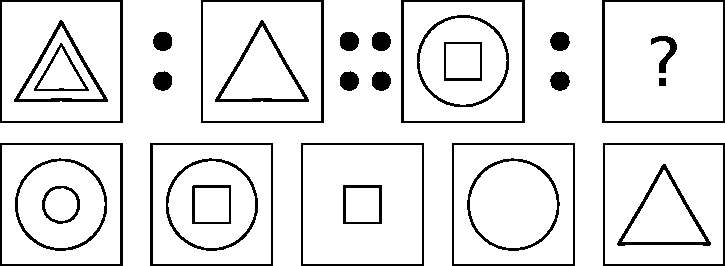
\includegraphics[width=0.7\textwidth]{figures/evans.pdf}
  \end{center}
  \begin{enumerate}
    \item Find high order relations
    \item Apply transformation $A \rightarrow B$ to $C \rightarrow D$
  \end{enumerate}
\end{frame}

\begin{frame}{Distance minimization in a vector space}
  Rumelhart \& Abrahamsen \cite{RumAbr73}: analogies between words
  \begin{center}
  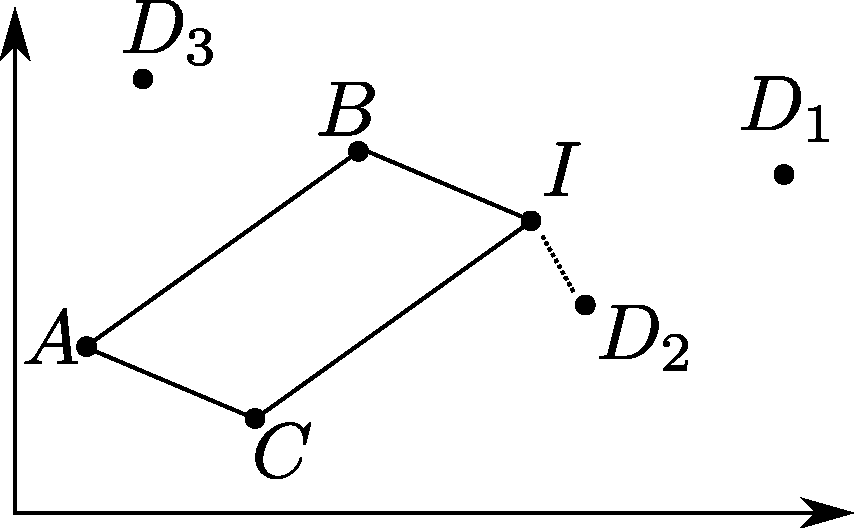
\includegraphics[width=0.5\textwidth]{figures/rumelhart_model.pdf}
  \end{center}
  \alert{Exactly} what \cite{BayMicDelIJCAI07} does
\end{frame}

\begin{frame}{Links with CBR}
  CBR:
\begin{itemize}
  \item Problem $P$, solution $S$ unkown
  \item Look for similar problems $P_i$ with known solutions $S_i$
  \item Make up $S$ from $\{S_i\}$
\end{itemize}

Our approach:
\begin{itemize}
  \item Find $3$-tuples such that $P_i: P_j :: P_k : P$
  \item Make up $S$ from $\{ \text{solutions to } S_i: S_j :: S_k : x\}$
\end{itemize}
  `Similar' $\rightarrow$ `\alert{adaptable}'. Frontiers and differences with
  analogical reasoning are really not that clear
\end{frame}

\section[Analogical proportions]{Formal models of analogical proportions}
%\subsection{Formal definitions}

\begin{frame}{3 axioms}
  \begin{center}
  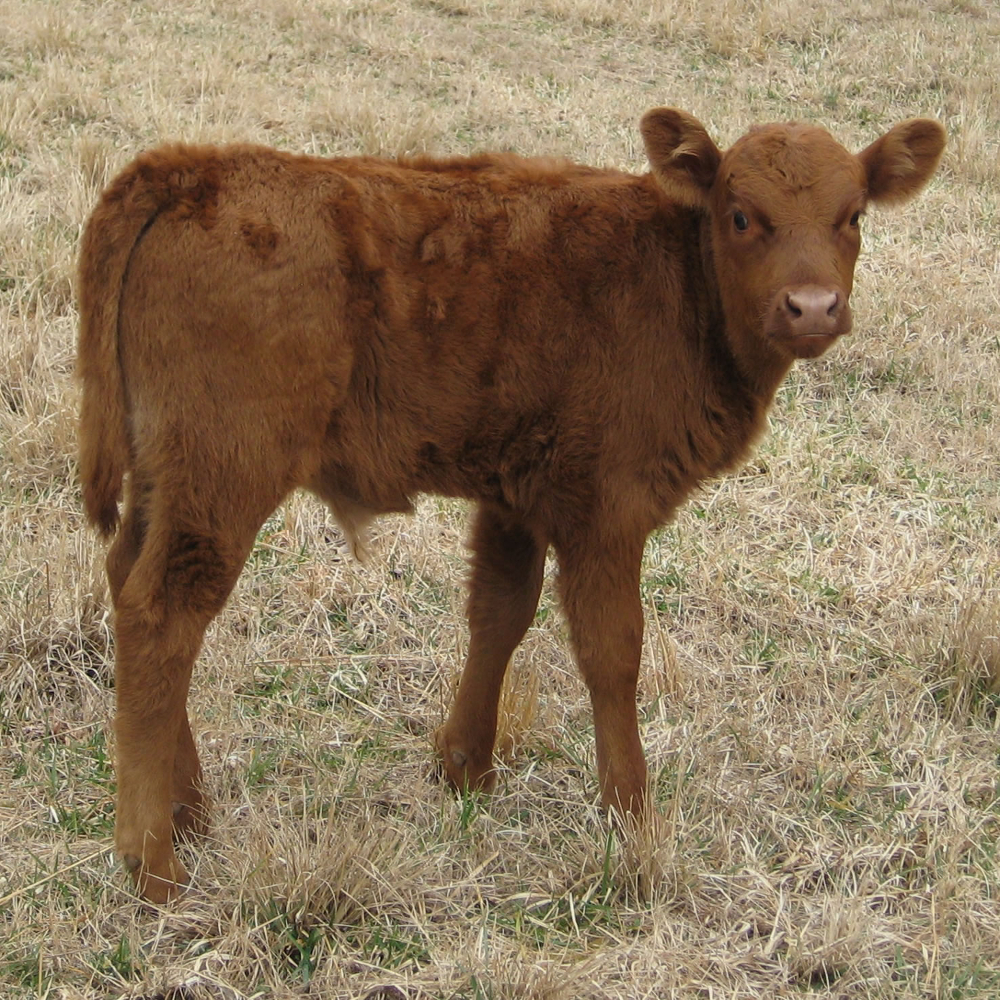
\includegraphics[width=0.1\textwidth]{figures/calf.jpg}
  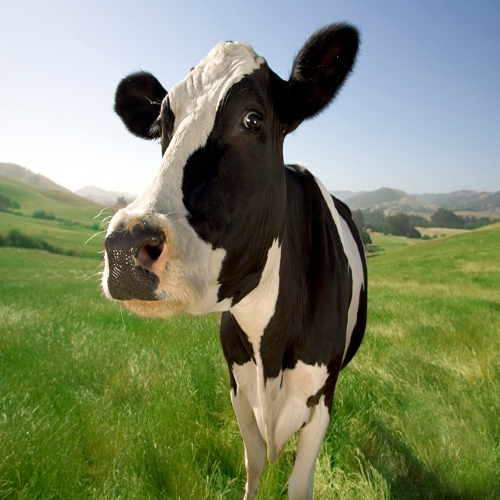
\includegraphics[width=0.1\textwidth]{figures/cow.jpg}
  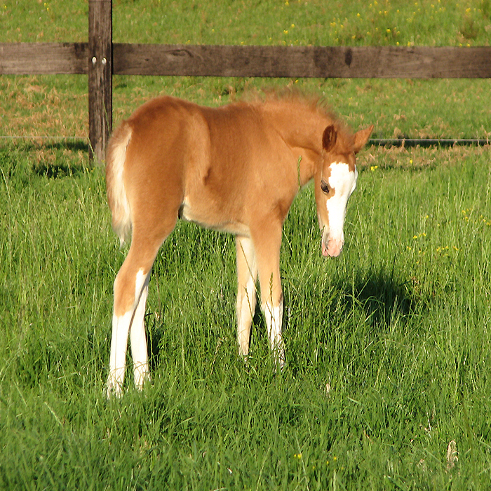
\includegraphics[width=0.1\textwidth]{figures/foal.jpg}
  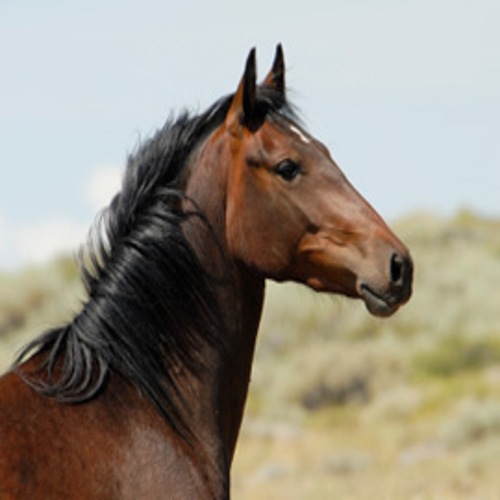
\includegraphics[width=0.1\textwidth]{figures/horse.jpg}
  \end{center}
  From Aristotle:
  \begin{enumerate}
    \item $a:b::a:b$ is always true
    \item $a:b::c:d \implies c:d::a:b$ (symmetry)
    \begin{center}
      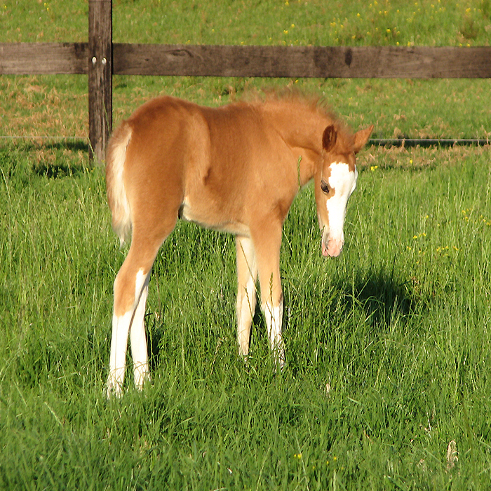
\includegraphics[width=0.1\textwidth]{figures/foal.jpg}
      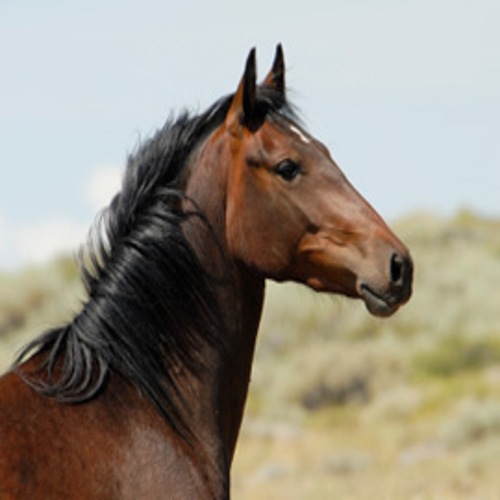
\includegraphics[width=0.1\textwidth]{figures/horse.jpg}
      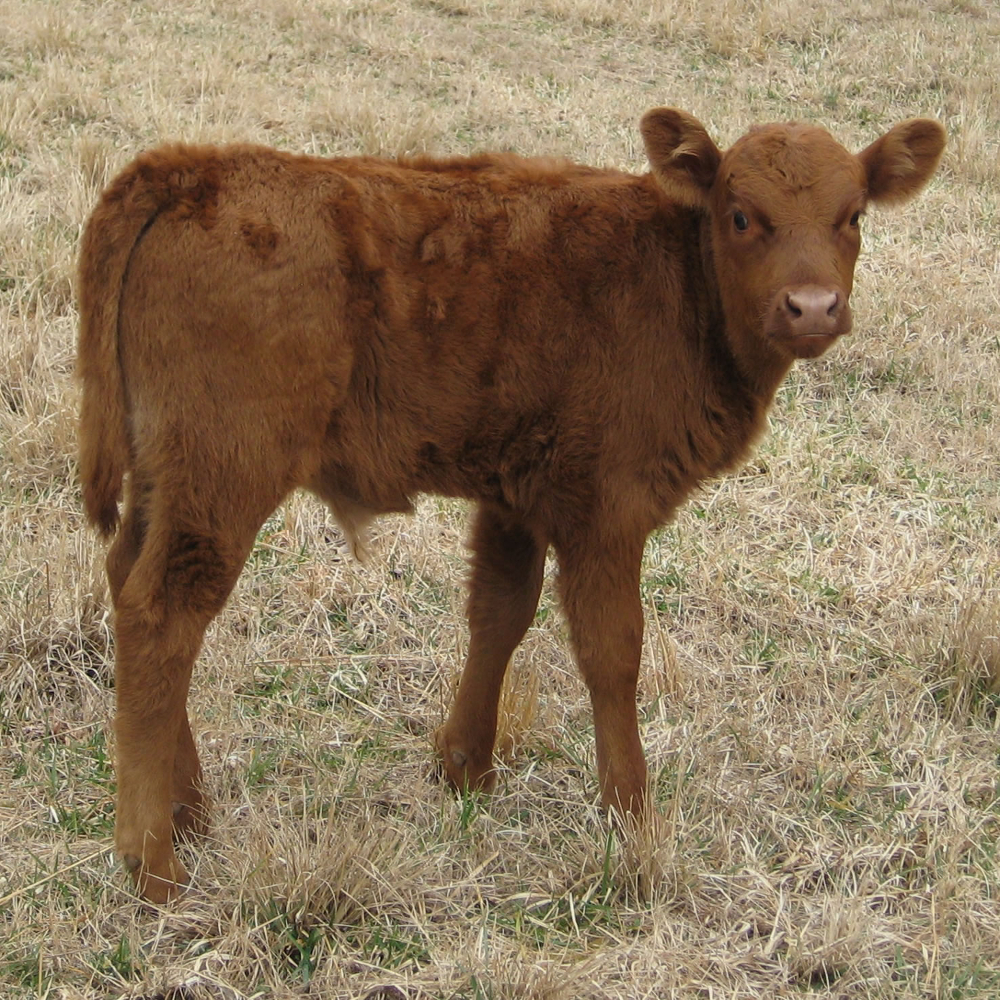
\includegraphics[width=0.1\textwidth]{figures/calf.jpg}
      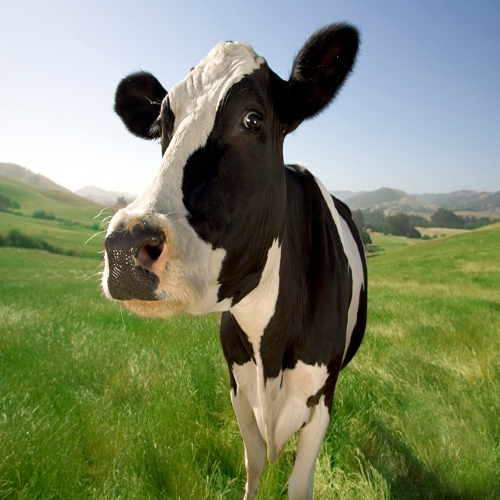
\includegraphics[width=0.1\textwidth]{figures/cow.jpg}
    \end{center}
    \item $a:b::c:d \implies a:c::b:d$ (central permutation)
    \begin{center}
      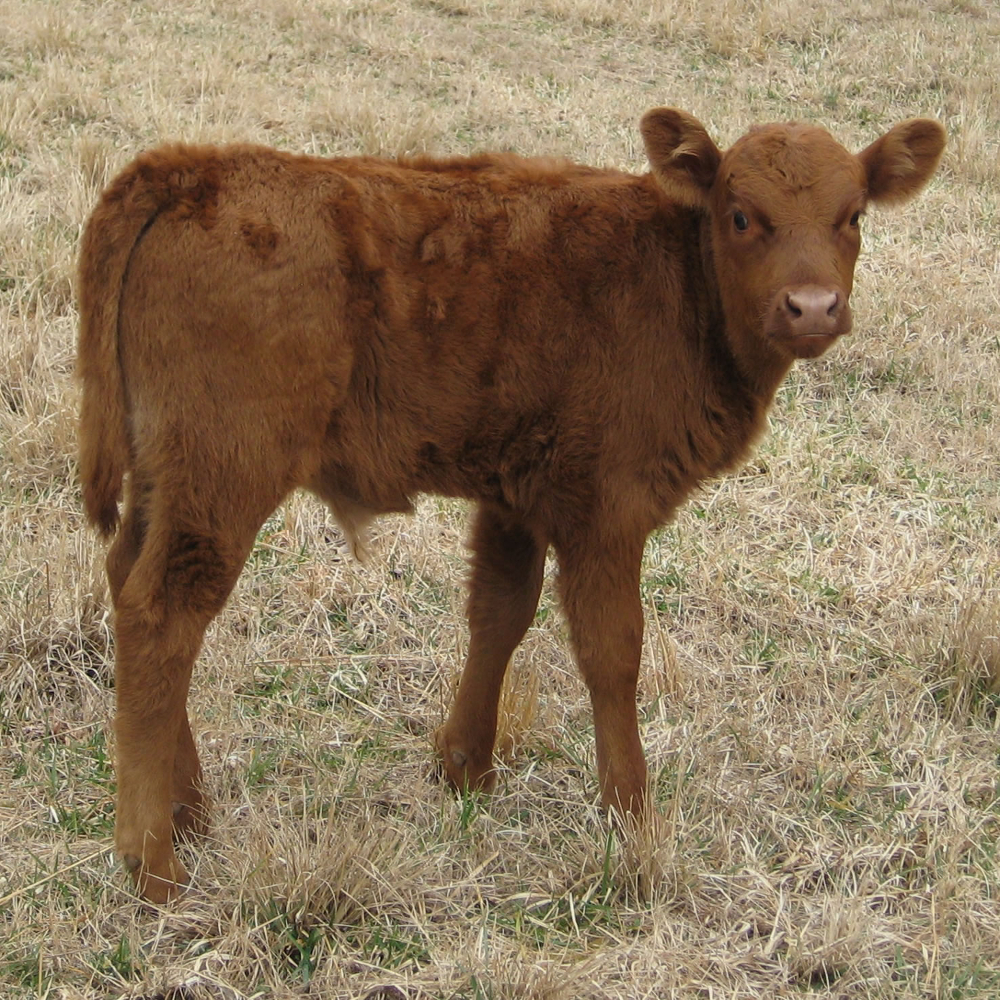
\includegraphics[width=0.1\textwidth]{figures/calf.jpg}
      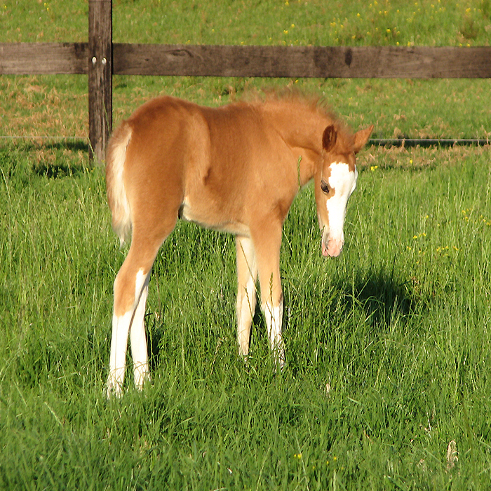
\includegraphics[width=0.1\textwidth]{figures/foal.jpg}
      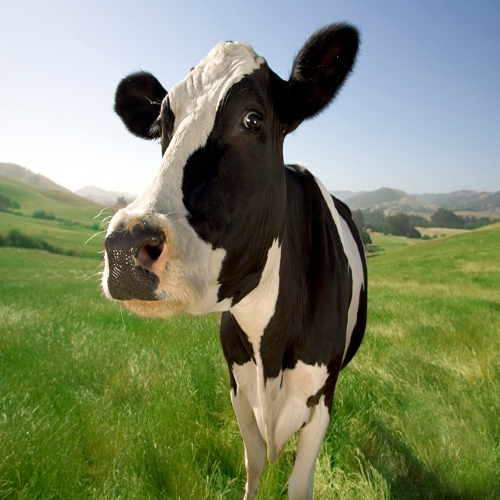
\includegraphics[width=0.1\textwidth]{figures/cow.jpg}
      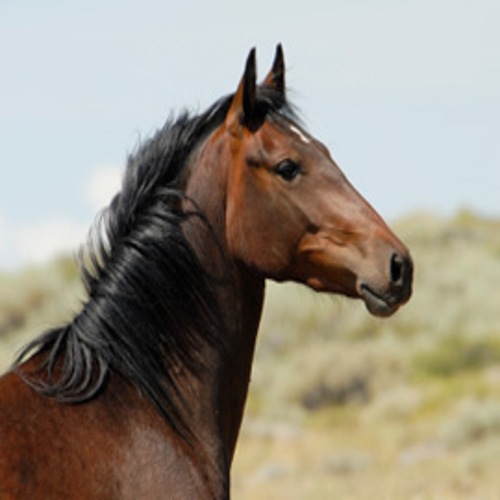
\includegraphics[width=0.1\textwidth]{figures/horse.jpg}
    \end{center}
  \end{enumerate}
\end{frame}

\begin{frame}{Proportions between numbers}
  \begin{itemize}
    \item Proportion in a group $(U, \oplus)$ \cite{StrYvoREPORT05}:
      $$a \oplus d = b \oplus c$$
    \item Geometric proportion $(\mathbb{R}, \times)$:
      $$a \times d = b\times c$$
    \item Arithmetic proportion $(\mathbb{R}, +)$:
      $$a + d = b + c \iff a - b = c - d$$
  \end{itemize}
\end{frame}

\begin{frame}{Proportion between vectors}
  Let $A$ be an analogy on $X$, $\mathbf{a}, \mathbf{b}, \mathbf{c}, \mathbf{d}
  \in X^m$
  $$A^m(\mathbf{a}, \mathbf{b}, \mathbf{c}, \mathbf{d}) ~ \text{  if  } ~
  A(a_i, b_i, c_i, d_i) \text{ for all } i \in [1, m]$$

  \begin{center}
    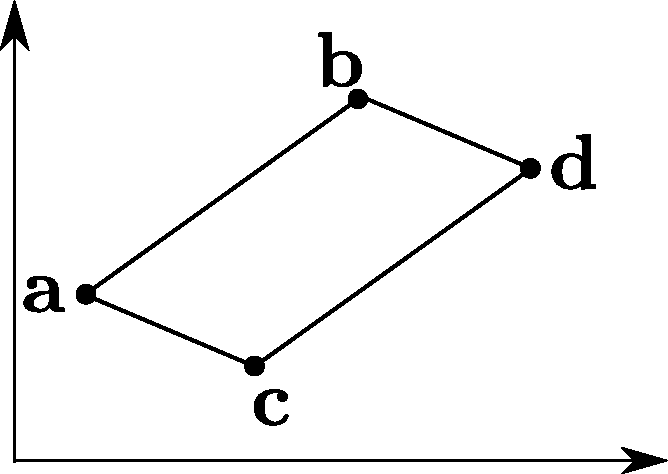
\includegraphics[width=.3\textwidth]{figures/arithmetic_proportion.pdf}
  \end{center}
\end{frame}

\begin{frame}{Boolean proportion}
  \begin{columns}
    \begin{column}{0.4\textwidth}
  $a, b, c, d \in \mathbb{B} = \{0, 1\}$ are in proportion if
  $$
  \begin{cases}
    a = b \text{ and } c = d\\
    \text{or}\\
    a = c \text{ and } b = d,
  \end{cases}
  $$
      \alert{
  or equivalently if
}
  $$a - b = c - d$$

      {\fontencoding{U}\fontfamily{futs}\selectfont\char 66\relax} $\mathbb{B}$
      is not closed for addition / subtraction
    \end{column}
    \begin{column}{0.4\textwidth}
  \begin{table}[t]
    \centering
    \begin{tabular}[t]{ccccc}
      \toprule
      $a$ & $b$ & $c$ & $d$ &  $A(a, b, c, d)$\\
      \midrule
      0 & 0 & 0 & 0 &   \textbf{1}\\
      1 & 1 & 1 & 1 &   \textbf{1}\\
      0 & 0 & 1 & 1 &   \textbf{1}\\
      1 & 1 & 0 & 0 &   \textbf{1}\\
      0 & 1 & 0 & 1 &   \textbf{1}\\
      1 & 0 & 1 & 0 &   \textbf{1}\\
      \bottomrule
    \end{tabular}
  \end{table}
    \end{column}
  \end{columns}
\end{frame}

\begin{frame}{Geometrical insights}
  \begin{center}
    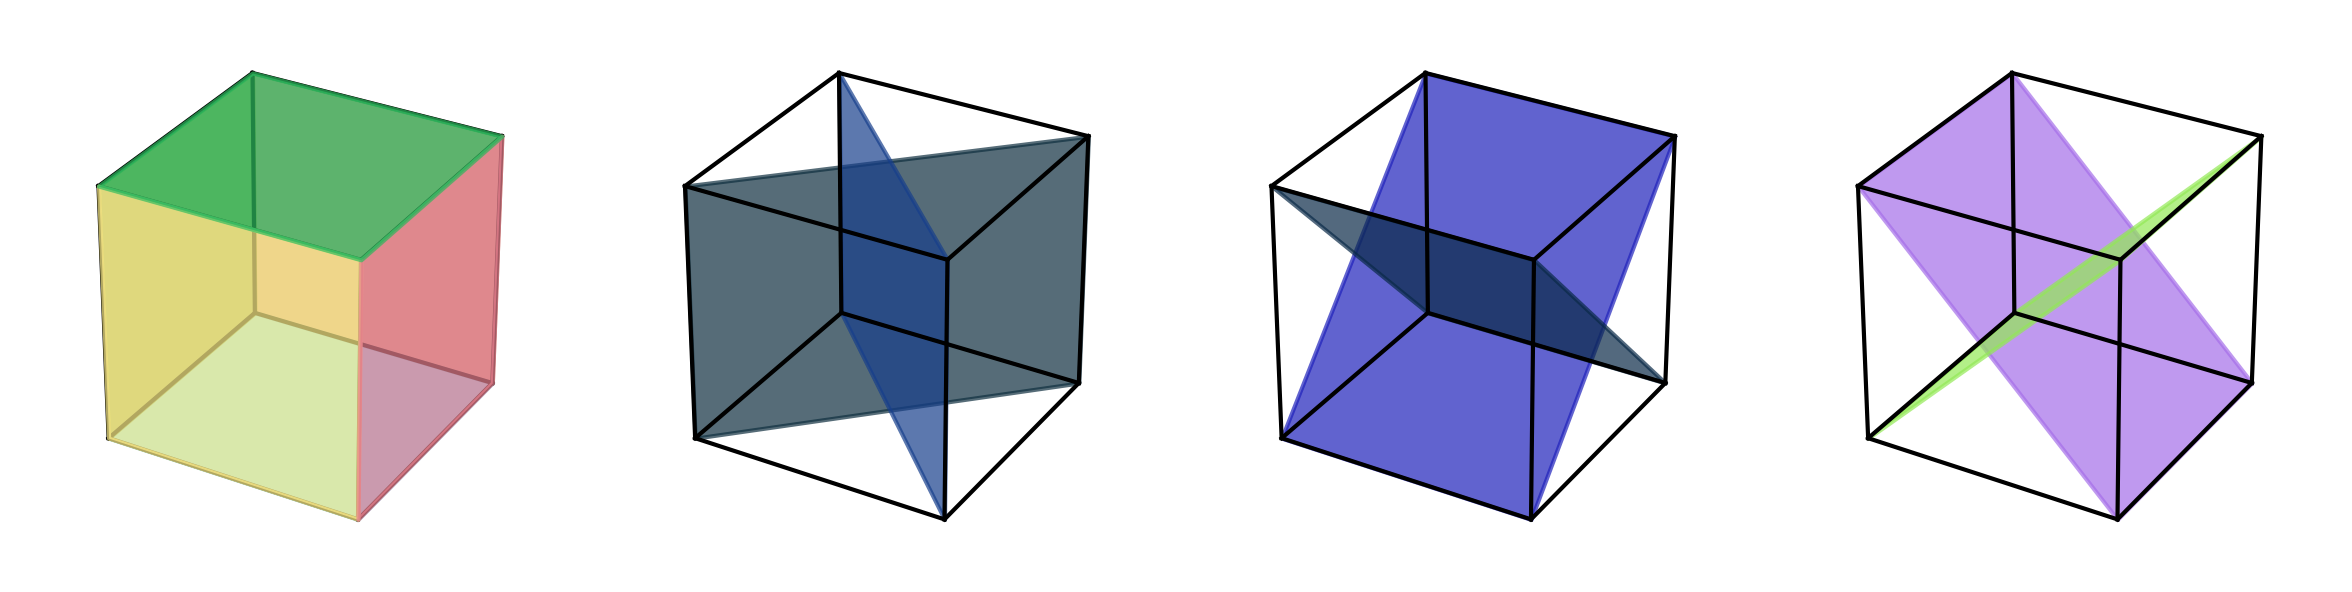
\includegraphics[width=0.9\textwidth]{figures/cubes_in_B3_pres.png}
  \end{center}
\end{frame}

%\subsection{Toy classification problem}
\begin{frame}{Problem}
  \begin{center}
    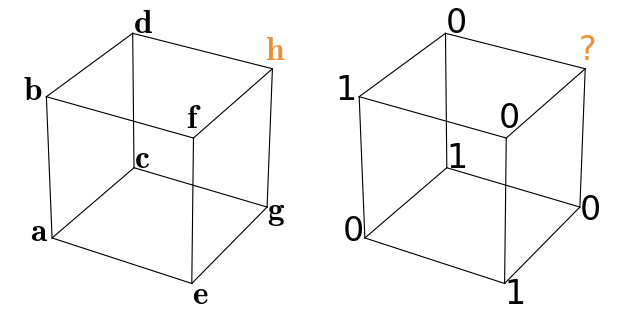
\includegraphics[width=0.9\textwidth]{figures/classification_problem_pres.png}
  \end{center}
\end{frame}

\begin{frame}{Inference principle, equation solving}
  \begin{columns}
    \begin{column}{0.4\textwidth}
      \begin{center}
        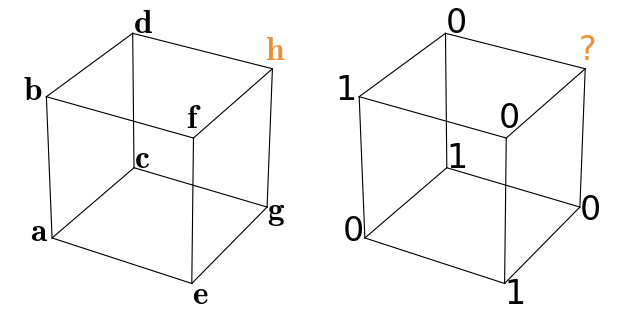
\includegraphics[width=0.9\textwidth]{figures/classification_problem_pres.png}
      \end{center}
      {\tiny
        \begin{table}[t]
          \centering
          \begin{tabular}[t]{cccc}
            \toprule
            $a$ & $b$ & $c$ & $\sol(a, b, c)$ \\
            \midrule
            0 & 0 & 0 & 0 \\
            1 & 1 & 1 & 1 \\
            0 & 0 & 1 & 1 \\
            1 & 1 & 0 & 0 \\
            0 & 1 & 0 & 1 \\
            1 & 0 & 1 & 0 \\
            1 & 0 & 0 &\times\\
            0 & 1 & 1 &\times\\
            \bottomrule
          \end{tabular}
        \end{table}
      }
    \end{column}
    \begin{column}{0.5\textwidth}
      $$
      \infer{\mathbf{x} : \mathbf{y} ::
      \mathbf{z} : \mathbf{t}}{f(\mathbf{x}) : f(\mathbf{y}) :: f(\mathbf{z}) :
      f(\mathbf{t})}
      $$
      \begin{itemize}
          \alert{
        \item $\mathbf{a} : \mathbf{b} :: \mathbf{g} : \mathbf{h}$
          \begin{itemize}
            \item $f(\mathbf{a}) : f(\mathbf{b}) :: f(\mathbf{g}) :~?$
            \item $0:1::0:~?$
            \item $\hat{f}(\mathbf{h}) = 1$
          \end{itemize}
            }
        \item $\mathbf{a} : \mathbf{d} :: \mathbf{e} : \mathbf{h}\rightarrow
          \hat{f}(\mathbf{h}) = 1$
        \item $\mathbf{a} : \mathbf{c} :: \mathbf{f} : \mathbf{h}\rightarrow
          \hat{f}(\mathbf{h}) = 1$
        \item $\mathbf{b} : \mathbf{d} :: \mathbf{f} : \mathbf{h}\rightarrow
          \times$\\(not solvable)
      \end{itemize}

    \end{column}
  \end{columns}
\end{frame}

\section[Analogical classification]{Analogical classification: a functional definition}

\begin{frame}{A few definitions}
  \begin{itemize}
    \item \alert{Analogical Extension}
        \begin{align*}
          \esf \eqdef \{ \mathbf{x} \in X^m |  &\exists
          (\mathbf{a},\mathbf{b},\mathbf{c}) \in S^3, ~ \mathbf{a} : \mathbf{b}
          :: \mathbf{c} : \mathbf{x}\\
          &\text{ and } f(\mathbf{a}) : f(\mathbf{b}) ::
          f(\mathbf{c}) : y \text{ is solvable}\}
        \end{align*}

      \item \alert{Analogical root}
      \begin{align*}
        \rsfx \eqdef \{(\mathbf{a}, \mathbf{b}, \mathbf{c}) \in S^3 |
        &\mathbf{a}:\mathbf{b}::\mathbf{c}:\mathbf{x}\\ &\text{ and }
        f(\mathbf{a}):f(\mathbf{b})::f(\mathbf{c}):y \text{ is solvable}\}
      \end{align*}

    \item \alert{Analogical label}
      $$\albl{\mathbf{x}} \eqdef \text{ most common solution }y$$
  \end{itemize}
\end{frame}

\begin{frame}{A few definitions -- examples}
  \begin{center}
    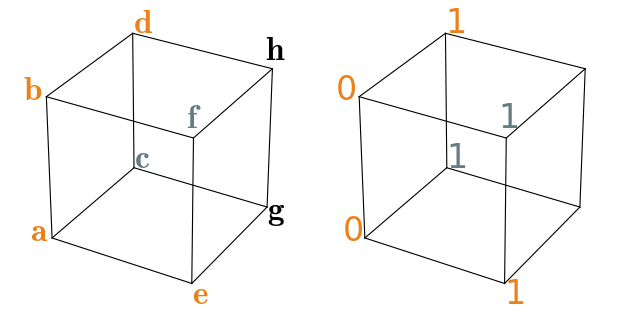
\includegraphics[width=.7\textwidth]{figures/ae_example_pres.png}
  \end{center}
  \begin{columns}
    \begin{column}{.5\textwidth}
      \begin{align*}
        &\textcolor{orange}{S = \Set{\mathbf{a}, \mathbf{b}, \mathbf{d}, \mathbf{e}}}\\
        &\textcolor{grey}{\esfs = \Set{\mathbf{c}, \mathbf{f}}}\\
        &\aroot{S}{f}{\mathbf{c}} = \Set{(\mathbf{b}, \mathbf{d},
        \mathbf{a})}\\
        &\aroot{S}{f}{\mathbf{f}} = \Set{(\mathbf{a}, \mathbf{b}, \mathbf{e})}
      \end{align*}
    \end{column}
    \begin{column}{.5\textwidth}
      \begin{align*}
        \albl{\mathbf{c}} &= 1\\
         \albl{\mathbf{f}} &= 1
      \end{align*}
    \end{column}
  \end{columns}
\end{frame}

\begin{frame}{Conservative classifier\cite{StrYvoREPORT05}}
  \begin{columns}
    \begin{column}{0.5\textwidth}
      \begin{itemize}
        \item Compute $\esf$, and $\albl{\mathbf{x}} ~~~ \forall \mathbf{x} \in \esf$
        \item $\forall x \in\esf, ~~ \hat{f}(\mathbf{x}) \eqdef \albl{\mathbf{x}}$
        \item $\forall x \notin \esf, ~~ \hat{f}(\mathbf{x})$ is undefined
      \end{itemize}
    \end{column}
    \begin{column}{0.5\textwidth}
      \begin{center}
        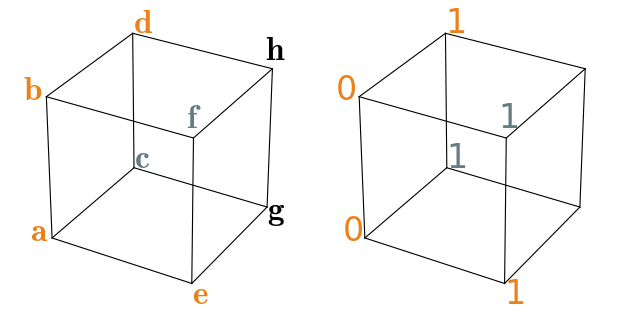
\includegraphics[width=.9\textwidth]{figures/ae_example_pres.png}
      \end{center}
      \begin{itemize}
      \item $\esfs = \Set{\mathbf{c}, \mathbf{f}}$
      \item $\hat{f}(\mathbf{c}) \eqdef \albl{\mathbf{c}} = 1$\\
        $\hat{f}(\mathbf{f}) \eqdef \albl{\mathbf{f}} = 1$
      \item $\hat{f}(\mathbf{g}) =~?, ~~~ \hat{f}(\mathbf{h}) =~?$
      \end{itemize}
    \end{column}
  \end{columns}
\end{frame}

\begin{frame}{Extended classifiers \cite{BayMicDelIJCAI07}}
  \begin{columns}
    \begin{column}{0.5\textwidth}
  Use \alert{analogical dissimilarity}
    \begin{enumerate}
      \item $\forall (\mathbf{a}, \mathbf{b}, \mathbf{c}) \in S^3$, compute
        $\AD(\mathbf{a}, \mathbf{b}, \mathbf{c}, \mathbf{x})$.
        Keep $k$ lowest values
      \item $\hat{f}(\mathbf{x}) =$ most common solution to $f(\mathbf{a}) :
        f(\mathbf{b}) :: f(\mathbf{c}) : y$.
    \end{enumerate}
      \begin{center}
        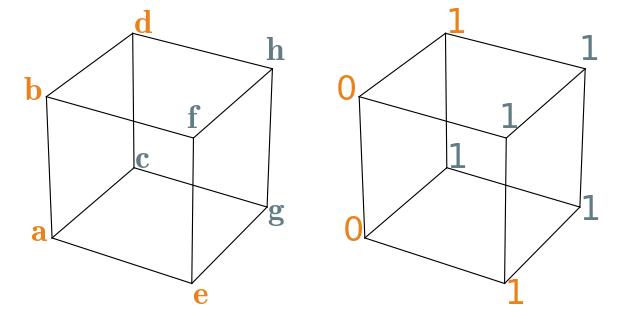
\includegraphics[width=.8\textwidth]{figures/ae_example2_pres.png}
      \end{center}
    \end{column}
    \begin{column}{0.5\textwidth}
      {\tiny
      $$
      \begin{array}{ccccc}
        \toprule
        a & b & c & d &  \AD(a, b, c, d)\\
        \midrule
        0 & 0 & 0 & 0 &   \textbf{0}\\
        0 & 1 & 0 & 1 &   \textbf{0}\\
        0 & 0 & 1 & 1 &   \textbf{0}\\
        0 & 0 & 0 & 1 &   \textbf{1}\\
        0 & 0 & 1 & 0 &   \textbf{1}\\
        0 & 1 & 0 & 0 &   \textbf{1}\\
        1 & 0 & 0 & 0 &   \textbf{1}\\
        0 & 1 & 1 & 0 &   \textbf{2}\\
        \bottomrule
      \end{array}
      $$
      }
      \begin{itemize}
      \item $\hat{f}(\mathbf{c}) = 1$ ~~~
        $\hat{f}(\mathbf{f}) = 1$
      \item $\hat{f}(\mathbf{g}) = 1$ ~~~
        $\hat{f}(\mathbf{h}) = 1$
      \end{itemize}
    \end{column}
  \end{columns}
\end{frame}

\begin{frame}{Rewriting analogical dissimilarity}

$$\AD(\mathbf{a},\mathbf{b},\mathbf{c},\mathbf{x})=\norm{}{\mathbf{x} -
(\mathbf{c}-\mathbf{a}+\mathbf{b})}=\norm{}{\mathbf{x} - \mathbf{d}}$$
\begin{center}
  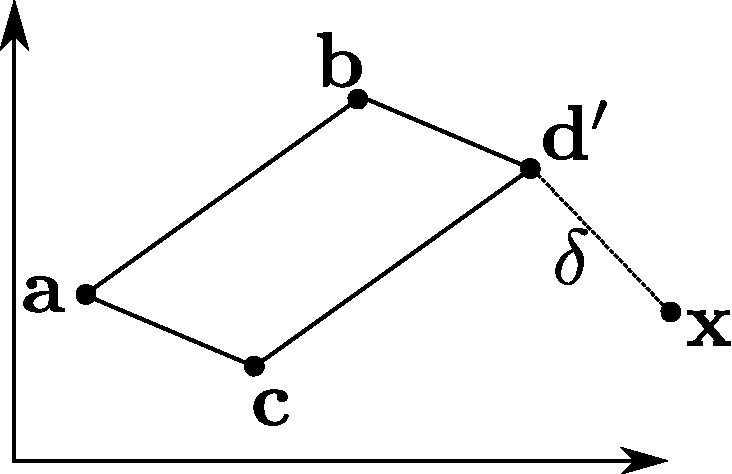
\includegraphics[width=.3\textwidth]{figures/analogical_dissimilarity_pres.pdf}
\end{center}

  With $S = \Set{\mathbf{a}, \mathbf{b}, \mathbf{c}}, \esf = \Set{\mathbf{a},
  \mathbf{b}, \mathbf{c}, \mathbf{x}}, ~~ \AD(\mathbf{a}, \mathbf{b},
  \mathbf{c}, \mathbf{x}) = \delta(\mathbf{d}, \mathbf{x})$

  and $\hat{f}(\mathbf{x}) = \albl{\mathbf{d}}$

  $\mathbf{d}$ is the \alert{nan} of $\mathbf{x}$
\end{frame}

\begin{frame}{Functional definition}
  \begin{columns}
    \begin{column}{.6\textwidth}
      $$
      k\text{-nan}\left(\mathbf{x}, S\right) \eqdef \Set{\argmin_{\mathbf{d} \in
      A_E^Y(S)}^k
      \delta(\mathbf{x},\mathbf{d})}
      $$
      $$\hat{f}(\mathbf{x}) \eqdef \text{Mode}\Set{\albl{\mathbf{d}} | \mathbf{d}
      \in k\text{-nan}\left(\mathbf{x}, S\right)}
      $$
      (Mode = Majority vote)
    \end{column}
    \begin{column}{.4\textwidth}
      \begin{center}
        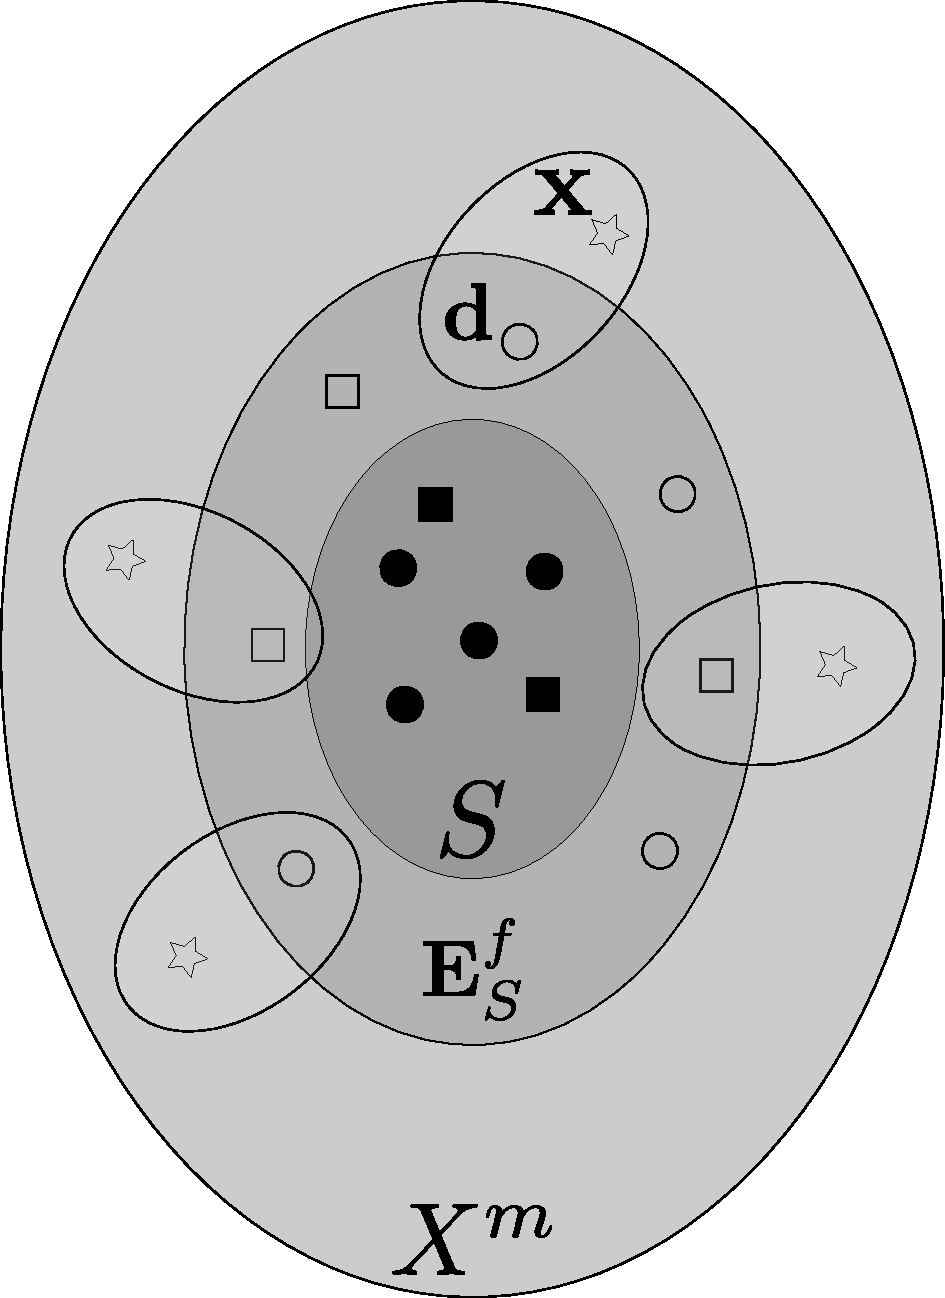
\includegraphics[width=.9\textwidth]{figures/extended_classifier_pres.pdf}
      \end{center}
    \end{column}
  \end{columns}
\end{frame}

\begin{frame}{A new perspective}
  \begin{columns}
    \begin{column}{.5\textwidth}
      \begin{enumerate}
        \item Extend $S$ to build $\esf$
        \item Run $k$-NN over $\esf$
      \end{enumerate}
    \end{column}
    \begin{column}{.5\textwidth}
      \begin{center}
        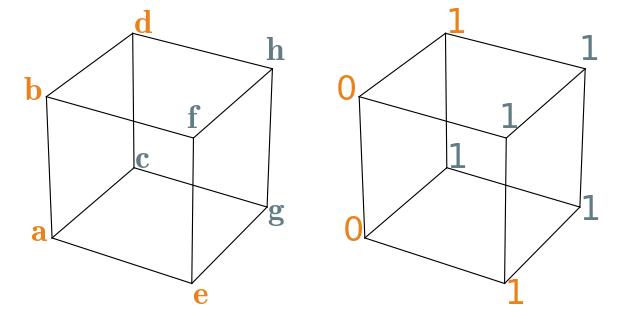
\includegraphics[width=.8\textwidth]{figures/ae_example2_pres.png}
      \end{center}
        \begin{align*}
          \hat{f}(\mathbf{c}) &= \albl{\mathbf{c}}\\
          \hat{f}(\mathbf{f}) &= \albl{\mathbf{f}}\\
          \hat{f}(\mathbf{g}) &= \text{Mode}\{f(\mathbf{e}), \albl{\mathbf{c}}\}\\
          \hat{f}(\mathbf{h}) &= \text{Mode}\{f(\mathbf{d}), \albl{\mathbf{f}}\}
        \end{align*}
    \end{column}
  \end{columns}
\end{frame}

\begin{frame}{Theoretical properties}
  \begin{itemize}
    \item $P\left(\lim_{n \to \infty} \nanemph(\mathbf{x}, S_n) =
      \mathbf{x}\right) = 1$
    \item VC-dim = $\infty$
    \item $\acc(\NAN_S, X^m) = ~\acc(\NN_S, A) \cdot \alpha ~ +
      \acc(\NN_{\esfs}, B) \cdot (1 - \alpha) $
    \begin{itemize}
    \item $A$: the elements that have their nan in $S$
    \item $B$: the elements that have their nan in $\esfs$
    \item $\alpha \eqdef P(\mathbf{x} \in A)$
  \end{itemize}
  \end{itemize}
\end{frame}

\section[Application to recommendation]{Analogical reasoning for recommendation}

\begin{frame}{Taxonomy}
  \begin{itemize}
    \item Content-based: leverage metadata about items
    \item \alert{Collaborative filtering}: leverage collaborative data
    \item Knowledge-based: leverage user requirements
  \end{itemize}
\end{frame}

\begin{frame}{Problem}
$$
R= \begin{pmatrix}
1 & \textcolor{orange}{?} & 2 & \textcolor{orange}{?} & \textcolor{orange}{?}\\
\textcolor{orange}{?} & \textcolor{orange}{?} & \textcolor{orange}{?} & \textcolor{orange}{?} & 4\\
2 & \textcolor{orange}{?} & 4 & 5 & \textcolor{orange}{?}\\
\textcolor{orange}{?} & \textcolor{orange}{?} & 3 & \textcolor{orange}{?} & \textcolor{orange}{?}\\
\textcolor{orange}{?} & 1 & \textcolor{orange}{?} & 3 & \textcolor{orange}{?}\\
5 & \textcolor{orange}{?} & \textcolor{orange}{?} & \textcolor{orange}{?} & 2\\
\end{pmatrix}
\begin{matrix}
\text{Alice}\\
\text{Bob}\\
\text{Charlie}\\
\text{Daniel}\\
\text{Eric}\\
\text{Frank}\\
\end{matrix}
$$

More than 99\% entries are missing
\begin{itemize}
  \item Predict the $\textcolor{orange}{?}$ with a prediction algorithm
  \item Recommend items based on the estimated ratings
\end{itemize}
\end{frame}

\begin{frame}{Analogical recommendation: predicting $\rui$}
  \begin{itemize}
    \item Look for $3$-tuples of users $(a, b, c)$ such that $r_{aj}: r_{bj} ::
      r_{cj} : r_{uj}$ for most items $j$
    \item $\predrui = \aggr{} r_{ci} - r_{ai} + r_{bi}$
    \begin{center}
      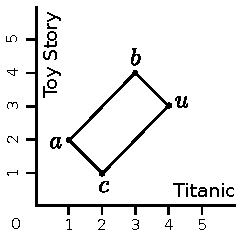
\includegraphics[width=0.2\textwidth]{figures/analogical_recommendation.pdf}
    \end{center}
  \item Comes with various tweaks
  \item \alert{Experiments}: close to neighborhood approach, but $\mathcal{O}(n^3)$
  \end{itemize}
\end{frame}

\begin{frame}{Alternative: clones}
    \begin{center}
      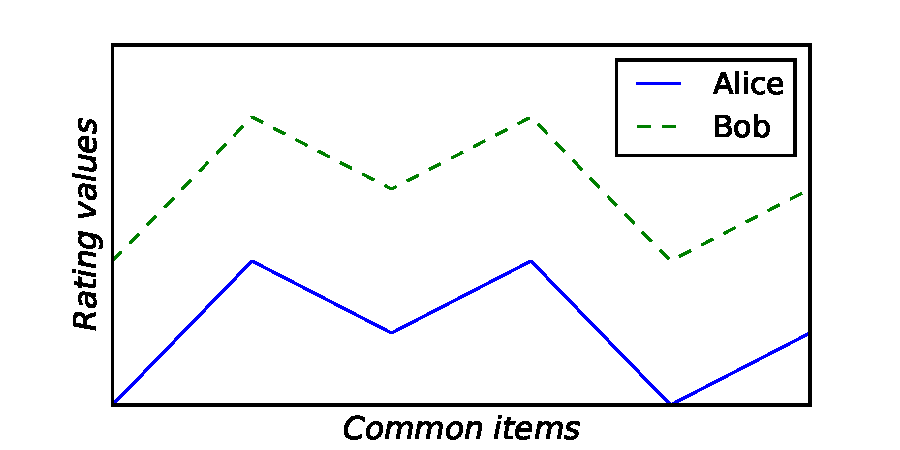
\includegraphics[width=0.4\textwidth]{figures/clones.pdf}
    \end{center}
    \begin{itemize}
      \item `Bruteforce' algorithm: drastic improvement on accuracy
      \item Capture clones in similarity measure: drastic improvement on
        computation time
      \item Already similar ideas in the literature
    \end{itemize}
\end{frame}

\begin{frame}{Mining analogical proportions}

  Looking for proportions in a rating matrix
  $$
    R= \begin{pmatrix}
    1 & ? & 2 & ? & ?\\
    ? & ? & ? & ? & 4\\
    2 & ? & 4 & 5 & ?\\
    ? & ? & 3 & ? & ?\\
    ? & 1 & ? & 3 & ?\\
    5 & ? & ? & ? & 2\\
    \end{pmatrix}
  $$

  Based on \alert{Apriori} algorithm:
  \begin{itemize}
    \item Find all $4$-itemsets with Apriori
    \item Filter them with a quality function
  \end{itemize}
\end{frame}

\begin{frame}{Examples}
  \resizebox{\textwidth}{!}{
  \begin{tabular}{l l  l  l l}
\toprule
    &\multicolumn{1}{c}{$i_1$}  & \multicolumn{1}{c}{$i_2$} &
    \multicolumn{1}{c}{$i_3$} & \multicolumn{1}{c}{$i_4$}\\
  \midrule
 1&   Star Wars & The Emp. Strikes Back & Raid. of the Lost Ark & Return of the Jedi  \\
 2&   Star Wars & Return of the Jedi & Raid. of the Lost Ark & The Emp. Strikes Back  \\
 3&   Star Wars & The Emp. Strikes Back & Return of the Jedi & Raid. of the Lost Ark  \\
 4&   Star Wars & Raid. of the Lost Ark & Return of the Jedi & I.J. and the Last Crus.  \\
 5&   Star Wars & Return of the Jedi & Raid. of the Lost Ark & The Fugitive  \\
 6&   Star Wars & Raid. of the Lost Ark & Return of the Jedi & Back to the Future  \\
 7&   Star Wars & The Emp. Strikes Back & Raid. of the Lost Ark & I.J. and the Last Crus.  \\
 8&   Star Wars & The Emp. Strikes Back & Return of the Jedi & I.J. and the Last Crus.  \\
 9&   Star Wars & The Emp. Strikes Back & I.J. and the Last Crus. & Return of the Jedi  \\
 10&   Star Wars & Raid. of the Lost Ark & The Emp. Strikes Back & The Fugitive\\
\bottomrule
\end{tabular}
}
\end{frame}

\begin{frame}{Examples}
  \resizebox{\textwidth}{!}{
  \begin{tabular}{ l l  l  l l }
\toprule
    &\multicolumn{1}{c}{$i_1$}  & \multicolumn{1}{c}{$i_2$} &
    \multicolumn{1}{c}{$i_3$} & \multicolumn{1}{c}{$i_4$}\\
  \midrule
  1&   To Catch a Thief  & Laura  & Gigi  & An American in Paris  \\
  2&   Nick of Time  & It Could Happen to You  & Milk Money & Only You  \\
  3& To Catch a Thief  & An American in Paris  & Gigi  & Meet John Doe   \\
  4& Dangerous Minds  & Money Train  & Higher Learning  & With Honors   \\
  5& Judge Dredd  & Under Siege 2: Dark Territory  & The Shadow  & Mortal Kombat   \\
  6& Terminal Velocity & Under Siege 2: Dark Territory  & Money Train  & Drop Zone    \\
  7& Judge Dredd  &Under Siege 2: Dark Territory  &  Mortal Kombat  & Coneheads   \\
  8& To Catch a Thief  & An American in Paris  & Gigi  & Laura   \\
  9&  To Catch a Thief  & Meet John Doe  & Gigi  & An American in Paris   \\
 10&   Nick of Time  & It Could Happen to You  & Only You  & Milk Money   \\
\bottomrule
\end{tabular}
}
\end{frame}

\begin{frame}{Take-away}
  \begin{itemize}
    \item Available proportions are a bit trivial
    \item Could explain results of first experiments (close to $k$-NN)
  \end{itemize}
\end{frame}

\section[AP functions]{Analogy-preserving functions}
\begin{frame}{A quick recap}
  \begin{columns}
    \begin{column}{.4\textwidth}
      Analogical classification:
      \begin{enumerate}
        \item Extend $S$ to build $\esf$
        \item Run $k$-NN over $\esf$
      \end{enumerate}
    \end{column}
    \begin{column}{.6\textwidth}
      \begin{itemize}
        \item No need to use $k$-NN
        \item How to ensure a sound extention?
        \item How to ensure that $\albl{\mathbf{x}} = f(\mathbf{x})$?
        \item \alert{How to make this valid?}
        $$
        \infer{\mathbf{x} : \mathbf{y} ::
        \mathbf{z} : \mathbf{t}}{f(\mathbf{x}) : f(\mathbf{y}) :: f(\mathbf{z}) :
        f(\mathbf{t})}
        $$
      \end{itemize}
    \end{column}
  \end{columns}
\end{frame}

\begin{frame}{It's not always a good idea}
  \begin{center}
    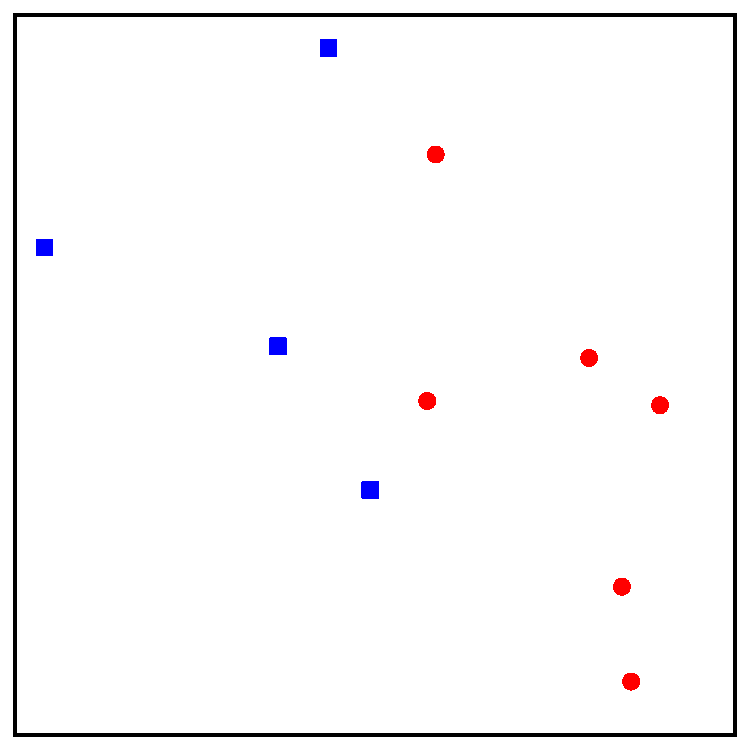
\includegraphics[width=.5\textwidth]{figures/AE_in_R2_S.pdf}
    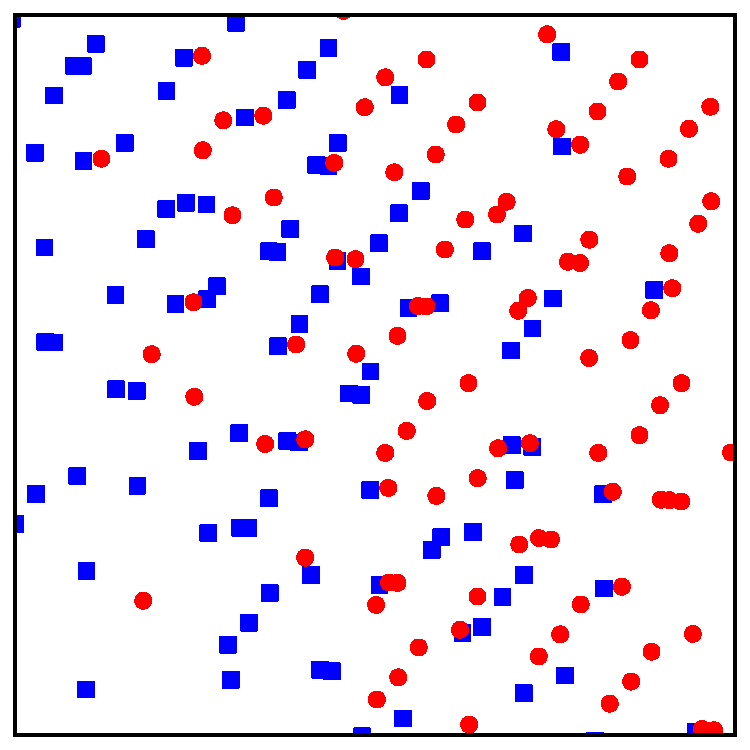
\includegraphics[width=.5\textwidth]{figures/AE_in_R2_AE.pdf}
  \end{center}
\end{frame}

\begin{frame}{Analogy preserving functions}
  $$
  \begin{cases}
    \mathbf{a} :  \mathbf{b} ::  \mathbf{c} :  \mathbf{d} \emph{ and }\\
    \emph{solvable}(f(\mathbf{a}), f(\mathbf{b}),  f(\mathbf{c}))
  \end{cases}
  \implies \emph{sol}\left(f(\mathbf{a}),  f(\mathbf{b}),  f(\mathbf{c})\right) =
  f(\mathbf{d})$$

  \alert{Main result}: AP functions are the Boolean affine functions (XOR
  functions):
  $$f(x_1,\ldots , x_m)=\alpha_1\cdot x_1+\ldots +\alpha_m\cdot x_m+\alpha_0$$

  \begin{center}
  `$+$' $\leftrightarrow$ XOR\\
  `$\cdot$' $\leftrightarrow $ AND
  \end{center}
\end{frame}

\begin{frame}{AP functions - affine functions}
  \begin{columns}
    \begin{column}{.5\textwidth}
      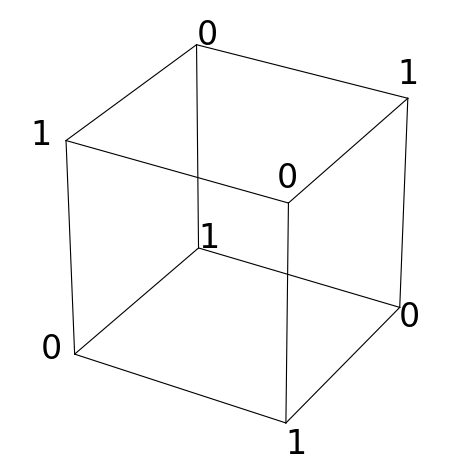
\includegraphics[width=.9\textwidth]{figures/affine_functions_neighbors.png}
    \end{column}
    \begin{column}{.5\textwidth}
      Proof sketch:
      \begin{enumerate}
        \item All Boolean functions are polynoms\\
          $f$ affine $\iff \text{deg}(f) < 2$
        \item $f$ affine $\implies$ $f$ AP
        \item $\text{deg}(f) \geq 2 \implies f$ not AP
      \end{enumerate}
    \end{column}
  \end{columns}
\end{frame}

\begin{frame}{Some extensions}
  \begin{itemize}
    \item Real case: AP functions $\approx$ affine functions
    \item Multiple-valued attributes: a bit trickier
    \item \alert{Approximate} AP functions: $\varepsilon$-close functions to
      $L$
      $$P(\omegasf \geq \eta) > 1 - \delta$$
     $$\omegasf \eqdef P\left(\albl{\mathbf{x}} = f(\mathbf{x}) \given[\big]
      \mathbf{x} \in \esfs\right)$$
      $$\textcolor{orange}{\eta = ?,~ \delta = ?}$$
  \end{itemize}
\end{frame}

\section*{Conclusion}

\begin{frame}{Contributions}
  \begin{itemize}
    \item Two algorithms for analogical recommendation (\alert{ISMIS'15},
      \alert{FuzzIEEE'16})
    \item An algorithm for analogical proportion mining (\alert{LFA'16})
    \item A Python RS engine (\url{http://surpriselib.com})
    \item Functional (unifying) definition of analogical classifiers
      (\alert{ECAI'16})
      \begin{itemize}
        \item Clear links with $k$-NN
        \item Convergence, VC-dim, accuracy
      \end{itemize}
    \item Characterization of functions leading to a perfect analogical
      extension (\alert{IJCAI'17})
  \end{itemize}
\end{frame}

\begin{frame}{Future works}
  \begin{itemize}
    \item Role of majority vote procedure
    \item Piecewise affine functions?
    \item Transfer learning?
    \item Approximate AP functions
      $$P(\omegasf \geq \eta) > 1 - \delta$$
  \end{itemize}
\end{frame}

\begin{frame}{That's it}
  \begin{center}
    Thanks!
  \end{center}
\end{frame}

\bibliographystyle{alpha}
\bibliography{biblio}

\end{document}
